\chapter{\IfLanguageName{dutch}{Stand van zaken}{State of the art}}
\label{ch:stand-van-zaken}

% Tip: Begin elk hoofdstuk met een paragraaf inleiding die beschrijft hoe
% dit hoofdstuk past binnen het geheel van de bachelorproef. Geef in het
% bijzonder aan wat de link is met het vorige en volgende hoofdstuk.

% Pas na deze inleidende paragraaf komt de eerste sectiehoofding.

As mentioned in the previous chapter, this research will go deeper into headless Drupal and attempt to figure out how to utilise it and why it became so popular. But before anwsering these questions it is important to have a clear understanding of what headless Drupal acually is. This will be discussed in this chapter. 

\section{Architectures}
A traditional CMS like Drupal in its base form consists of a monolithic architecture. This means that the CMS offers anything a user would need in a web application, including a database, back-end and front-end.

When going headless, the architecture of the CMS goes from monolithic to the so-called decoupled architecture. In this form, only the back-end and database that the CMS offers are utilised. Then, instead of distributing the content in this back-end to one channel, it can be consumed by different channels, including web applications made with front-end frameworks like React and Angular, but even mobile applications.

Monolithic and decoupled are the two main architectures that are considered when using a CMS, but there are two other architectures worth mentioning: the fully decoupled static site and progressively decoupled ~\autocite{Dropsolid2021}. The latter two are less well known, but are still important to look at to get the whole picture of what headless is. All of these architectures will be discussed in this chapter.

\subsection{Monolithic or Traditional}
The traditional or monolithic architecture is the one used by all traditional CMSs out of the box. It means that the application is one big end-to-end system. For Drupal in particular, this means that the theming functions which encompass the front-end are completely coupled and dependent on Drupal's back-end.

This architecture has both upsides and downsides. One big upside is that this is a very robust and reliable system. The system is predictable and easy to use. The downside to this architecture is that it has led to something often called Drupalisms on the front-end ~\autocite{So2018}. This means that some terminology and features specific to Drupal came to exist, which are hard to understand for developers less familiar with Drupal. 

One other negative is that this system can feel limiting for front-end developers, because they have to work within the boundaries of the specific theme they are using.

\begin{figure}
\centering
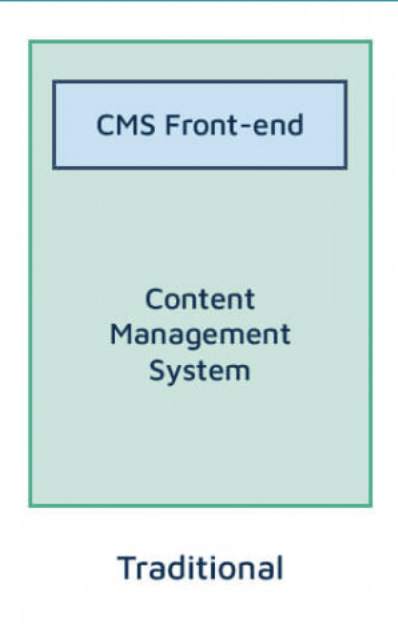
\includegraphics{./img/Traditional_Architecture}
\caption[Traditional CMS architecture]{A representation of the traditional or monolithic architecture ~\autocite{Dropsolid2021}}
\end{figure}

\subsection{Headless or Decoupled}

The fully decoupled or headless architecture is the one that has become more and more popular over the years ~\autocite{Dropsolid2021}. Decoupled means that the components of the system don't depend on each other like they do with the monolithic architecture ~\autocite{So2018}. They interact with each other using web services instead.

Fully decoupling the back-end from the front-end is the most well known type of decoupled out there. It allows developers much more freedom to choose any technology they want to build the presentation layer (front-end) of the application.

This approach is the one that will be discussed further in this research.

\begin{figure}
	\centering
	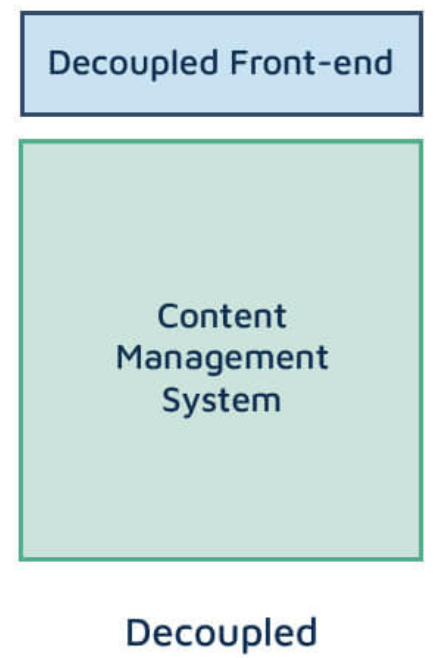
\includegraphics{./img/Headless_Architecture}
	\caption[Headless CMS architecture]{A representation of the decoupled or headless architecture ~\autocite{Dropsolid2021}}
\end{figure}


\subsection{Fully decoupled static site}

The main difference this architecture has with the previous one is that content is not stored by the CMS itself. The content is instead maintained inside the front-end framework that is used. This is done using Hypertext Markup Language (HTML), Cascading Stylesheets (CSS) and Javascript (JS) files ~\autocite{Dropsolid2021}.

The big advantage of this approach is that performance and security are segnificantly enhanced, while also reducing the complexity for developers.

The approach with this kind of architecture is generally consists of retrieving content from the CMS with a static site generator, after which the static website is deployed to a Content Delivery Network (CDN) which, according to ~\textcite{Buyya2008}, is a "collaborative collection of network elements spanning the Internet, where content is replicated over
several mirrored Web servers in order to perform transparent and effective delivery of content to the end users".

\subsection{Progressively decoupled}

When using a progressively decoupled approach, the back-end of the CMS is not completely decoupled from the front-end. Instead, a javascript front-end framework is integrated, interwoven into the existing CMS front-end. This means that the Drupal front-end is still kept and not entirely replaced, unlike in the other two decoupled approaches. 

\begin{figure}
	\centering
	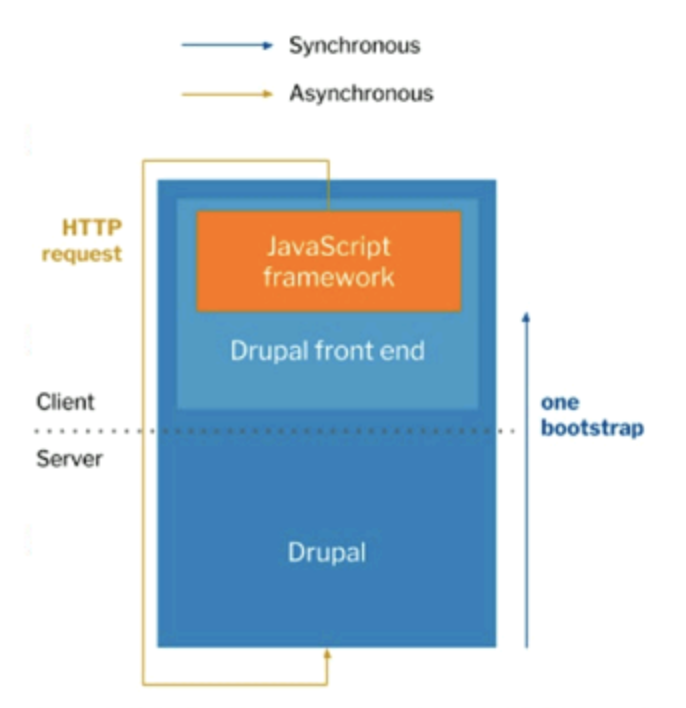
\includegraphics{./img/Progressively_Decoupled.png}
	\caption[Progressively decoupled CMS architecture]{A representation of the progressively decoupled architecture ~\autocite{So2018}}
\end{figure}

\section{RESTful Web Services}
\subsection{Basics of REST}
Representational State Transfer or REST is, according to~\textcite{Wilde2011}, \emph{"A set of constraints that inform the design of a hypermedia system"}. It is an architectural style with a set of guiding principles. These principles are: 
\begin{enumerate}
	\item Uniform Interface: All interactions are to be made around an interface that supports all these interactions.
	\item  Stateless: All interactions between a client and server need to be independent from one another.
	\item Client-Server: User-interface or client concerns are to be seperated strictly from back-end and data, or server related concerns.
	\item Layered System: Seperate components should not be allowed to see any layer beyond the layer they are interacting with.
	\item Caching: Any resources should allow for caching by the client, the server and any other components.
\end{enumerate}

\begin{figure}
	\centering
	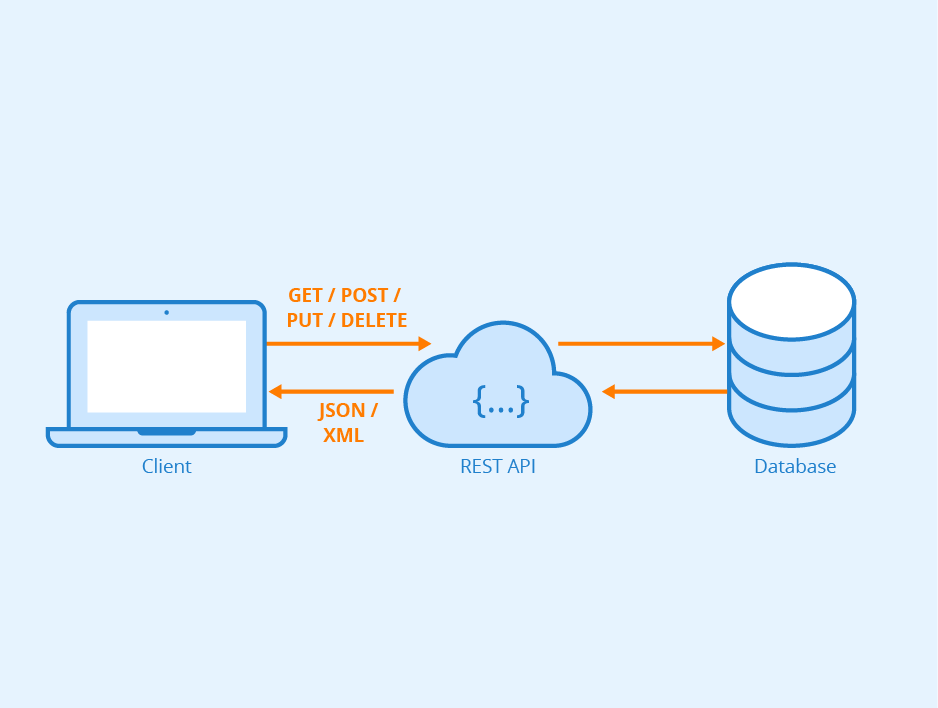
\includegraphics{./img/Rest-API.png}
	\caption[REST API]{A representation of a REST API ~\autocite{Seobility}}
\end{figure}

\subsection{Web services in Drupal 9}
Within Drupal 9 there exist two main ways of going headless. The most straightforward of the two is the JSON:API module. The other, which requires more configuration, is the Drupal core RESTful web services module.



